\chapter{Algorithm Selection Model Training Algorithms}

\section{Introduction}
This chapter explains the implementation details of the algorithms used in training the AS model, which are \textit{pairwise random forest regression} (PRFR) and REINFORCE.

\section{Data Preparation}
\label{sec:dataprep}

Table \ref{tbl:graphs2015} displays the summary on GRAPHS-2015 dataset.

\begin{table}[H]
	\centering
	\begin{tabular}{|l|l|}
		\hline
		\textbf{Scenario ID} & GRAPHS-2015 \\ \hline
		\textbf{Source} & \citet{graphs2015} \\ \hline
		\textbf{Number of problem instances} & 5725 \\ \hline
		\textbf{Number of features} & 35 \\ \hline
		\textbf{Number of algorithms} & 7 \\ \hline
		\multirow{7}{*}{\textbf{Algorithm list}} & LAD \\ \cline{2-2} 
		& SupplementalLAD \\ \cline{2-2} 
		& VF2 \\ \cline{2-2} 
		& GLASGOW1 \\ \cline{2-2} 
		& GLASGOW2 \\ \cline{2-2} 
		& GLASGOW3 \\ \cline{2-2} 
		& GLASGOW4 \\ \hline
		\textbf{Performance measure} & Runtime (in milliseconds) \\ \hline
	\end{tabular}
	\caption{GRAPHS-2015 dataset summary}
	\label{tbl:graphs2015}
\end{table}

Only a subset of GRAPHS-2015 was used for training AS models. A technique called \textit{presolving} is used to eliminate the quickly solvable problem instances, leaving the harder problem instances for AS. The steps on removing presolved instances from GRAPHS-2015 were discussed in PORTSUB study. The flow and code is shown in Figures \ref{fig:presolver} and \ref{fig:extracthard}.

\begin{figure}[H]
	\centering
	\scalebox{.85}{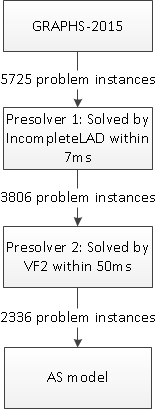
\includegraphics{./img/presolver.png}}
	\caption[Filtering presolved instances from GRAPHS-2015]{Filtering presolved instances from GRAPHS-2015. 2336 hard problems are left for AS.}
	\label{fig:presolver}
\end{figure}

\begin{figure}[H]
	\centering
	\scalebox{.60}{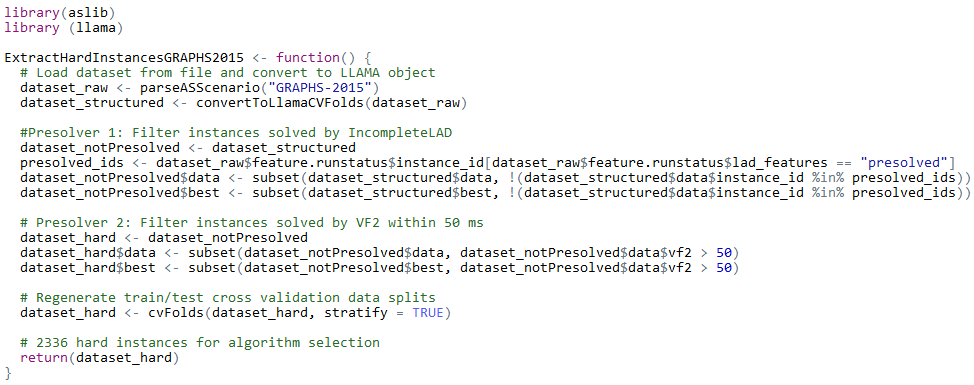
\includegraphics{./img/extract_hard_instances.png}}
	\caption{R script for extracting hard instances from GRAPHS-2015}
	\label{fig:extracthard}
\end{figure}

\section{Pairwise Random Forest Regression}
The AS model used in PORTSUB study was trained using a supervised learning approach called PRFR. It works as follows: for each pair of algorithms in the algorithm portfolio, a model is trained to predict the performance difference between them. If the first algorithm is better than the second, the difference is positive, otherwise negative. The algorithm with the highest cumulative performance difference, i.e. the most positive difference over all other algorithms, is chosen to be run. 

The LLAMA R package contains an implementation of pairwise random forest regression written by Lars Kotthoff, one of the PORTSUB authors. Its usage in R is shown on Figure \ref{fig:prfr}

\begin{figure}[H]
	\centering
	\scalebox{.65}{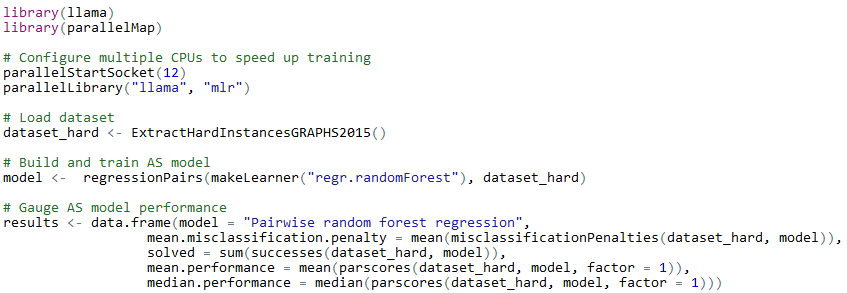
\includegraphics{./img/prfr.png}}
	\caption{R script for building AS model trained using PRFR}
	\label{fig:prfr}
\end{figure}

\section{REINFORCE}

The adaptation of REINFORCE algorithm to AS is composed of three main components:

\begin{enumerate}
	\item \textbf{Function approximator} \\
	An AS model can learn how algorithms match to problems with certain features. Patterns in problem features can be captured by function approximation methods, which translate feature values into parameters. For example, a simple function approximator such as linear regressor parameterizes inputs into slope and offset coefficients. Neural networks, a universal function approximator, represent parameters as network weights. Function approximation assists in generalizing AS model learning through discovery of feature patterns across problem instances.
	
	\item \textbf{Policy function} \\
	A policy function takes function approximator parameters as input and computes a probability for each algorithm. Algorithm probabilities change with respect to problem features. The computed probabilities serve as the basis of selection among algorithms.   
	
	\item \textbf{Reward function} \\
	The reward value is equivalent to the observed performance of the selected algorithm. It serves as feedback to the AS model to improve its capability in predicting optimal algorithms. Optionally, the reward value can be normalized or transformed to control how much the policy behavior should change with respect to feedback.  
\end{enumerate}

Figure \ref{fig:reinforce_flowchart} illustrates how an AS model is trained using \textit{REINFORCE} algorithm. 

\begin{figure}[H]
	\centering
	\scalebox{.65}{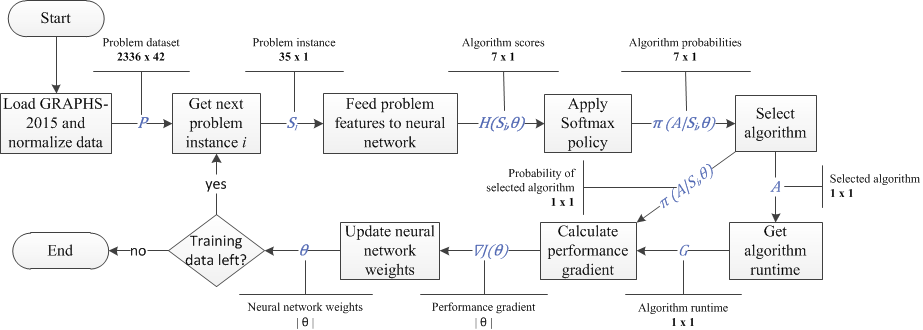
\includegraphics{./img/REINFORCE_flowchart.png}}
	\caption{Implementation of AS model trained using REINFORCE}
	\label{fig:reinforce_flowchart}
\end{figure}

\begin{enumerate}
	\item The GRAPHS-2015 dataset is loaded into R workspace. Hard problem instances are extracted, which consists of 2336 problem instances with 42 attributes used for training: 35 problem features plus runtime data of 7 algorithms.
	 
	\begin{figure}[H]
		\centering
		\scalebox{.75}{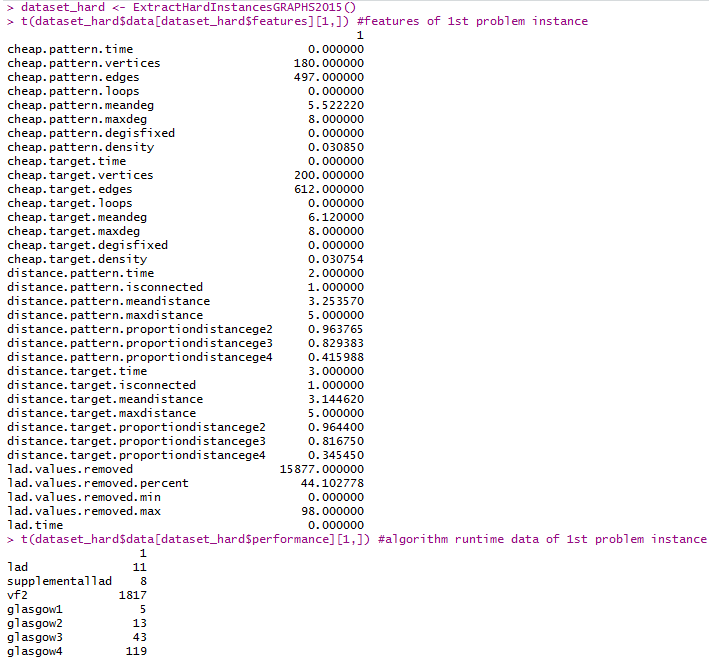
\includegraphics{./img/problem_instance.png}}
		\caption{Sample problem instance from GRAPHS-2015 dataset}
		\label{fig:problem_instance}
	\end{figure}

	\item Problem features are normalized using \textit{Z-score}. Normalization standardizes the range of data inputs which helps in resolving numerical issues when gradients are calculated during backpropagation. In effect, this speeds up neural network learning.
	
	\begin{equation}
	z_{ij} = \frac{x_{ij} - \mu_j}{\sigma_j}
	\end{equation} 
	
	where:
	
	\begin{table}[H]
		\centering
		\begin{tabular}{rl}
			$z_{ij} =$ & normalized feature value\\
			$x_{ij} =$ & feature value \\
			$\mu_{j} =$ & mean of \textit{jth} feature across \textbf{P} problem instances \\
			$\sigma_j =$ & standard deviation of \textit{jth} feature across \textbf{P} problem instances \\
			$\mathit{i} =$ & \textit{ith} instance from \textbf{P} problem instances \\
			$\mathit{j} =$ & \textit{jth} feature out of 35 features \\			
		\end{tabular}
	\end{table}

	The algorithm runtime data is rescaled to simplify the reward value used for computing the performance gradient. This enables the AS model to learn the most important information during problem solving, which is the ranking of algorithm performance from best to worst. This information is more important than the knowledge of actual algorithm runtimes, as the objective of AS is mainly not to characterize individual algorithm performance, but to determine which algorithms work best on problems. Table \ref{tbl:rewardscaling} shows how this study mapped algorithm ranking (determined by sorting runtime from shortest to longest) to reward values.

	\begin{table}[H]
		\centering
		\begin{tabular}{|c|c|}
			\hline
			\multicolumn{1}{|l|}{\textbf{Algorithm rank}} & \multicolumn{1}{l|}{\textbf{Assigned Reward Value}} \\ \hline
			1 & 16 \\ \hline
			2 & 4 \\ \hline
			3 & 1 \\ \hline
			4 & -4 \\ \hline
			5 & -16 \\ \hline
			6 & -64 \\ \hline
			7 & -256 \\ \hline
		\end{tabular}
		\caption{Algorithm ranking reward values}
		\label{tbl:rewardscaling}
	\end{table}
	
	\item A neural network is trained to map problem features (input) to algorithm scores (output). It is composed of an input layer with 35 inputs, 3 hidden layers, and an output layer with 7 outputs. Algorithm scores represent selection preferences, i.e., the larger the score, the more often that algorithm is taken.
	
	\item The algorithm scores are converted into probabilities using the softmax policy function. The probability assigned to an algorithm is proportional to its score, i.e., algorithms with the highest scores are given the highest probabilities of being selected. The softmax equation is given in the Equation below:
	
	\begin{equation}
	\pi(A | S_i, \theta) = \frac{\exp{H_A(S_i, \theta)}}{\sum_{b=1}^{7}\exp{H_b(S_i, \theta)}}
	\end{equation}
	
	where:
	
	\begin{table}[H]
		\centering
		\begin{tabular}{rl}
			$\pi(A | S_i, \theta) =$ & Probability of algorithm A \\
			$H_A(S_i, \theta) =$ & Algorithm score of algorithm A \\
			$H_B(S_i, \theta) =$ & Algorithm score of algorithm B \\
			$S_i =$ & features of problem instance \textit{i} \\
			$\theta =$ & neural network weights
		\end{tabular}
	\end{table}

	\item An algorithm is randomly selected based from the probabilities generated from the softmax policy function.
	
	\item The rescaled reward value corresponding to the selected algorithm is read from the dataset. This value, along with the probability of the selected algorithm, is used to calculate the performance gradient:
	
	\begin{equation}
	\nabla J(\theta_t) = G_t\ln{\pi(A | S_i, \theta_t)}
	\end{equation}
	
	where:
	
	\begin{table}[H]
		\centering
		\begin{tabular}{rl}
			$\nabla J(\theta_t) =$ & performance gradient \\
			$G_t =$ & reward \\
			$\pi(A | S_i, \theta_t) =$ & Probability of selected algorithm
		\end{tabular}
	\end{table}

	\item The performance gradient is used for backpropagation, a standard method of updating the weights of a neural network. Through this process, the neural network learns to adjust the algorithm scores in proportion to the reward value associated with the selected algorithm. 
	
	\begin{equation}
	\theta_{t+1} \gets \theta_t + \alpha \nabla J(\theta_t)
	\end{equation}
	
	where:
	
	\begin{table}[H]
		\centering
		\begin{tabular}{rl}
			$\theta_{t+1} =$ & Updated neural network weights \\
			$\theta_t =$ & current neural network weights \\
			$\alpha =$ & learning rate \\
			$\nabla J(\theta_t) =$ & performance gradient
		\end{tabular}
	\end{table}
\end{enumerate}

\section{Model Evaluation}
The performance of PRFR and REINFORCE are evaluated using 10-fold cross validation. The 2336 hard instances from GRAPHS-2015 are randomly partitioned into 10 subsets of approximately equal size. Of the 10 subsets, 9 are combined to form the training set for the AS models, while the remaining subset is formed as a test set. Mean MCP (Equation \ref{eq:mcp}) is calculated on the test set to evaluate the AS model performance. This is repeated 10 times for all possible combinations of training and test sets. At the end of this process, the final mean MCP is calculated by averaging the mean MCPs from all test sets.

\section{R source code implementation}
The implementation of AS models in this study can be retrieved from here: \url{https://github.com/kvrigor/algosel-rl}